%%%%%%%%%%%%%%%%%%%%%%%%%%%%%%%%%%%%%%%%%%%%%%%%%%%%%%%%%%%%
%%% LIVECOMS ARTICLE TEMPLATE FOR BEST PRACTICES GUIDE
%%% ADAPTED FROM ELIFE ARTICLE TEMPLATE (8/10/2017)
%%%%%%%%%%%%%%%%%%%%%%%%%%%%%%%%%%%%%%%%%%%%%%%%%%%%%%%%%%%%
%%% PREAMBLE
\documentclass[9pt,bestpractices]{livecoms}
% Use the 'onehalfspacing' option for 1.5 line spacing
% Use the 'doublespacing' option for 2.0 line spacing
% Use the 'lineno' option for adding line numbers.
% The 'bestpractices' option for indicates that this is a best practices guide.
% Omit the bestpractices option to remove the marking as a LiveCoMS paper.
% Please note that these options may affect formatting.

\usepackage{lipsum} % Required to insert dummy text
\usepackage[version=4]{mhchem}
\usepackage{siunitx}
\DeclareSIUnit\Molar{M}
\usepackage[italic]{mathastext}
\newcommand{\versionnumber}{0.1}  % you should update the minor version number in preprints and major version number of submissions.
\newcommand{\githubrepository}{\url{https://github.com/MobleyLab/basic_simulation_training}}  %this should be the main github repository for this article
\graphicspath{{figures/}}


%%%%%%%%%%%%%%%%%%%%%%%%%%%%%%%%%%%%%%%%%%%%%%%%%%%%%%%%%%%%%%%%%%%%%
%% Place any additional macros here.  Please use \newcommand* where
%% possible
%%%%%%%%%%%%%%%%%%%%%%%%%%%%%%%%%%%%%%%%%%%%%%%%%%%%%%%%%%%%%%%%%%%%%
\usepackage[colorinlistoftodos]{todonotes}
\usepackage{enumitem} % better handling
\usepackage{pifont} % some unicode-eqsue characters 


%%%%%%%%%%%%%%%%%%%%%%%%%%%%%%%%%%%%%%%%%%%%%%%%%%%%%%%%%%%%
%%% ARTICLE SETUP
%%%%%%%%%%%%%%%%%%%%%%%%%%%%%%%%%%%%%%%%%%%%%%%%%%%%%%%%%%%%
\title{Best Practices for Foundations in Molecular Simulations : v\versionnumber}

\author[1*]{Avisek Das}
\author[2]{David Mobley}
\author[1]{Heather Mayes}
\author[3]{Jacob I. Monroe}
\author[4]{Eliseo Marin-Rimoldi}
\author[5]{Samarjeet Prasad}
\author[6]{Justin Gilmer}
\author[7]{Jessica A. Nash}
%\author[2\authfn{1}\authfn{4}]{Firstname Initials Surname}
%\author[2*]{Firstname Surname}
\affil[1]{University of Michigan}
\affil[2]{University of California, Irvine}
\affil[3]{University of California, Santa Barbara}
\affil[4]{Univ 4}
\affil[5]{National Institutes of Standard and Technology}
\affil[6]{Vanderbilt University}
\affil[7]{Univ 7}

%\corr{email1@example.com}{FMS}  % Correspondence emails.  FMS and FS are the appropriate authors initials.
%\corr{email2@example.com}{FS}

%\contrib[\authfn{1}]{These authors contributed equally to this work}
%\contrib[\authfn{2}]{These authors also contributed equally to this work}

%\presentadd[\authfn{3}]{Department, Institute, Country}
%\presentadd[\authfn{4}]{Department, Institute, Country}

\blurb{This LiveCoMS document is maintained online on GitHub at
\githubrepository; to provide feedback, suggestions, or help improve it, please
visit the GitHub repository and participate via the issue tracker.}

%%%%%%%%%%%%%%%%%%%%%%%%%%%%%%%%%%%%%%%%%%%%%%%%%%%%%%%%%%%%
%%% ARTICLE START
%%%%%%%%%%%%%%%%%%%%%%%%%%%%%%%%%%%%%%%%%%%%%%%%%%%%%%%%%%%%

\begin{document}
\begin{frontmatter}
\maketitle

\begin{abstract}
This document provides a starting point for approaching molecular simulations, guiding beginning practitioners to what issues they need to know about before and while starting their first simulations, and why those issues are
so critical. 
This document makes no claims to provide an adequate introduction to the subject on its own. Instead, our goal is to help people know what issues are \emph{critical} before beginning, and to provide references to good resources on those topics. 
We also provide a checklist of key issues to consider before and while setting up molecular simulations which may serve as a foundation for other best practices documents.
\end{abstract}
\end{frontmatter}

\todo[inline, color={yellow!20}]{DLM: Authors editing should insert their info in the authors list above.}

% List TODOs here
\todototoc
\listoftodos

\section{Introduction}
\label{sec:intro}

\todo[inline, color={yellow!20}]{DLM: We should go through and break all the
material so that each sentence is on a separate line. This plays much nicer with
GitHub's version control, otherwise anytime anyone changes a word in a paragraph
it will look like the paragraph was completely rewritten...}

Molecular simulation techniques play a very important role in our quest for understanding the properties, structure, and function of molecular systems from a microscopic point of view.
Simulation methods are extremely useful for studying the structure and dynamics of complex systems that are too complicated for pen and paper theory and helping interpret experimental data in terms of molecular motions, as well as (increasingly) for quantitative prediction of properties of use in molecular design and other applications.

The basic idea of any molecular simulation method is quite simple; a particle-based description of the system under investigation is constructed and then the system is propagated by either deterministic or probabilistic rules to generate a trajectory. 
Relevant properties can be calculated for each ``snapshot'' (a stored configuration of the system, also called a ``frame'') and averaged over the the entire trajectory to compute estimates of desired properties.

Depending on how the system is propagated, molecular simulation methods can be divided into two main categories: Molecular Dynamics (MD) and Monte Carlo (MC).
With MD methods, the equation of motion is numerically integrated and a dynamical trajectory of the system is generated. 
MD simulations can be used for investigating structural, dynamic, and thermodynamic properties of the system.
With MC methods, probabilistic rules are used to generate a new configuration from the present configuration and this process is repeated to generate a sequence of states that can be used to calculate structural and thermodynamic properties but not dynamical properties; indeed, MC simulations lack any concept of time. 
Thus, the ``dynamics'' produced by an MC method is not the temporal dynamics of the system, in the sense that it may or may not follow the physical time evolution of the system. 
However, MC can be used to study dynamical behavior in model systems or in systems where MD simulations cannot be carried out due to computational cost, with a suitable mapping between MC step-size and a physical unit of time. 
This foundational document will focus on the concepts needed to carry out correct MD simulations that utilize good practices. 
Many, but not all, of the concepts here are also useful for MC simulations.

Either method can be carried out with different underlying physical theories to describe the particle-based model of the system under investigation.
If a quantum mechanics (QM) description of matter is used, electrons are explicitly represented in the model and interaction energy is calculated by solving the electronic structure of the molecules in the system with no (or few) empirical parameters, but with various approximations to the physics for tractability.  In a classical description, the molecules are represented by particles representing atoms or groups of atoms.  Each atom may be assigned an electric charge and a potential energy function with a large number of empirical parameters (fitted to experiment, QM, or other data)  is used to calculate non-bonded as well bonded interactions.
Classical simulations are much faster than quantum simulations, making them the methods of choice for vast majority of molecular simulation
studies on biomolecular systems in the condensed phase.
\todo[inline, color={red!20}]{Put in a few-sentence discussion re the size \& timescales of systems and the appropriate method; perhaps like the images often in papers; what are typical sizes and timescales that are tractable? This of course changes with time, but this is a living document so we're good. Also add in general, that the topology does not change--most FF do not allow chemical reactions}

For the rest of this document we will restrict ourselves to classical Molecular
Dynamics.

\section{Scope of this document}
\label{sec:scope}
There are several excellent textbooks on classical simulation methods; some of them are listed below.

\begin{itemize}
\item Allen and Tildesley
\item Frenkel, Smit and Geissler
\item Tuckermann
\end{itemize}

In principle, anyone with adequate prior knowledge should be able to pick up one of these books and learn the required skills to perform molecular simulations.
In practice, due to the interdisciplinary and somewhat technical nature of this field, many newcomers may find it difficult and time consuming to understand all the methodological issues involved in a simulation study.  
The goal of this document is to introduce a new practitioner to the basic concepts and bare minimum scientific knowledge required for correct execution of these methods. 
We also provide a basic set of ``best practices'' that can be used to avoid common errors, missteps and confusion in elementary molecular simulations work.

Modern implementations of classical simulations rely on a large body of knowledge from the fields of computer science and numerical methods, which will
not be covered in detail here.
However, in conducting and analyzing the results of such simulations, it is very helpful if one is comfortable using a Linux environment and command line \todo[inline, color={red!20}]{Insert link to background info}, as well as writing basic scripts in a variety of programming languages. A working knowledge of these topics is assumed; readers without such knowledge should be prepared to study on these topics when needed.



\section{Science topics}
\label{sec:science}
A variety of fields provide the foundation for our simulation methods and analysis of the data produced by these methods.
A new practitioner does not have to be an expert of all these fields but needs to understand some key concepts from each of these disciplines.
Here are topics we believe even basic users of molecular simulations need to grasp.

\subsection{Classical mechanics}
\label{sec:classical_mechanics}
\subsubsection{Key concepts}
\begin{itemize}
\item Newton's equations of motion and constants of motion
\item Hamilton's equations
\item Point particles and rigid bodies
\item Holonomic constraints
\end{itemize}

Molecular simulation methods work on many particles systems following the rules of classical mechanics. Basic knowledge of key concepts of classical mechanics is important for understanding simulation methods.
Molecular models are made of point particles with mass and electric charge.
These models have internal degrees of freedom like real molecules, for example reasonable descriptions of deformation of bond lengths and bond angles are provided by the models and simulation methods. 
Sometimes it is much more efficient to freeze the internal degrees of freedoms and treat the molecule as a rigid body where the particles
do not change their relative orientation as the whole body moves; this is commonly done, for example, for rigid models of the water molecule.
Due to the high frequency of the O-H vibrations, accurately treating water classically would require a very small time step, so for computational efficiency water is often instead treated as a rigid body.
Implementation of rigid bodies in a simulation protocol  involves holonomic constraints, where the rigidity is defined by imposing a minimal set of fixed bond lengths and angles through iterative procedures during the numerical integration of the equation of motion.
It is important to understand the concept of point particle, rigid bodies and constraints.

Classical mechanics has several mathematical formulations namely Newtonian, Hamiltonian and Lagrangian. These formulations are equivalent and produce same results but for certain applications one formulation can be more appropriate
than the other. 
Many simulation methods use the Hamiltonian formulation and therefore basic knowledge of Hamiltonian mechanics is essential.
Classical mechanics has several conserved quantities, for example, the total energy of the
system is a constant of motion.
These concepts play very important role is development and proper implementation of simulation methods.
For example, the most straightforward check of the correctness of an MD code is to test the quality of the energy conservation.

\subsubsection{Books}
\begin{itemize}
\item Most books on molecular simulations have a short discussions or appendices on classical mechanics that can serve the purpose of very quick introductions to the basic concepts.
For more detailed treatments of key concepts relevant for molecular simulations, consult specific chapters of Goldstein, Poole and Safko as mentioned below.

\item Goldstein, Poole and Safko. Chapter 1 gives a general introduction to basic concepts, chapter 2 discusses Lagrangian formulation, chapters 4 and 5 deals with rigid body motions, which is an important concept in molecular simulation. For Hamiltonian formulation consult chapter 8.
\end{itemize}

\subsubsection{Online resources}


\subsection{Thermodynamics}
\label{sec:thermodynamics}
\subsubsection{Key concepts}
\begin{itemize}
\item Temperature, pressure, stress
\item Internal energy, enthalpy
\item Gibbs and Helmholtz free energy
\item Entropy
\end{itemize}

One of the main objectives of molecular simulations is to estimate/predict thermodynamic behavior of real systems. 
It is important to understand key concepts in thermodynamics, such as temperature, pressure, internal energy, various forms of free energy and relationship between them. 
Basic properties of these quantities should be faithfully mimicked by simulation methods. 
It is quite straightforward to calculate internal energy, temperature and pressure from simulations, and these calculations can serve as quick sanity checks for the simulation setup. 
Clear understanding of these concepts is absolutely essential for grasping certain technical aspects of MD simulations namely, thermostat and barostat, which will be discussed in later sections. 
Basic thermodynamic principles also dictate proper simulation protocols and associated best practices.

\subsubsection{Books}
Equilibrium thermodynamics is taught in most undergraduate programs in physics, chemistry, biochemistry and various engineering disciplines.
Depending on the background, the practitioner can choose one or more of the following books to either learn or refresh their basic knowledge of thermodynamics. 
\begin{itemize}
\item Atkins' physical chemistry book \cite{AtkinsBook} : chapters 1 to 4.
\item Zemansky and Dittman \cite{ZemanskyBook}: Chapters 1 to 4, 5, 8 and 15.
\end{itemize}
\subsubsection{Online resources}

\subsection{Classical statistical mechanics}
\label{sec:stat_mech}
\subsubsection{Key concepts}
\begin{itemize}
\item Ensembles, distribution functions for different ensembles. Equivalence of ensembles
\item What equilibrium means and difference between equilibrium and
    non-equilibrium.
    For instance, what is usually called an ``equilibrium trajectory'' generally will not embody a good sample of the equilibrium ensemble due to insufficient sampling.  
        On the other hand, truly non-equilibrium conditions such as driven transitions and relaxation are fundamentally different. 
        Note that relaxation can occur to the equilibrium ensemble or a non-equilibrium condition (e.g., steady state).
\item Clarify differences between nonequilibrium ensembles: driven
    nonequilibrium steady-state, systems driven out of equilibrium by a time-dependent field, systems initially out of equilibrium but relaxing
        to equilibrium
\item Time averages and ensemble averages
\item Fluctuations
\item Correlation functions
\end{itemize}
\subsubsection{Books}
\begin{itemize}
\item Reif
\item McQuarrie
\item Dill
\item Hill
\item Shell
\item Zuckerman
\item Kaznessis
\end{itemize}
\subsubsection{Online resources}
\begin{itemize}
\item David Kofke's notes: \url{http://www.eng.buffalo.edu/~kofke/ce530/Lectures/lectures.html}
\item Scott Shell's notes: \url{https://engineering.ucsb.edu/~shell/che210d/assignments.html}
\end{itemize}

\subsection{Classical electrostatics}
\label{sec:classical_electrostatics}
\subsubsection{Key concepts}

%\item Long range nature of the Coulomb interaction
Electrostatic interactions are both some of the longest-range interactions in molecular systems and the strongest, with the interaction (often called
``Coulombic'' after Coulomb's law) between charged particles falling off as $1/r$ where $r$ is the distance separating the particles. 
In classical molecular simulations, atoms are typically represented by sites bearing charge in units of fractions of an elementary charge, so atom-atom interactions are thus necessarily long range compared to other interactions in these systems (which fall off a $1/r^3$ or faster).  
This means atoms or molecules separated by considerable distances can still have quite strong electrostatic interactions, though this also depends on the degree of shielding of the intervening medium (or its relative permittivity or dielectric constant).

%\item Polarizability, dielectric constants
The static dielectric constant of a medium, or relative permittivity $\epsilon_r$ (relative to that of vacuum), affects the prefactor for the decay of these long range interactions, with interactions falling off as $\frac{1}{\epsilon_r}$. 
Water has a relatively high relative permittivity or dielectric constant close to 80, whereas non-polar compounds such as n-hexane may have relative permittivities near 2 or even lower. 
This means that interactions in non-polar media such as non-polar solvents, or potentially even within the relatively non-polar core of a larger molecule such as a protein, are effectively much longer-range even than those in water. 
The dielectric constant of a medium also relates to the degree of its electrostatic response to the presence of a charge; larger dielectric constants correspond to larger responses to the presence of a charge in proximity.

It turns out that atoms and molecules also have their own levels of electrostatic response; particularly, their electron distributions polarize in response to their environment, effectively giving them an internal dielectric constant. 
This polarization can be modeled in a variety of ways, such as (in fixed charge force fields) building in a fixed amount of polarization which is thought to be appropriate for simulations in a generic ``condensed phase'' or by explicitly including polarizability via QM or by building it into a simpler, classical model which includes polarizability such as via explicit atomic polarizabilities [ref Amoeba, etc.] or via Drude oscillator-type approaches, where inclusion of extra particles attached to atoms allows for a type of effective polarization.
\todo[inline,
color={yellow!20}]{DLM: Add references.}

%\item why/when we need Ewald-type sums
Because so many interactions in physical systems involve polarity, and thus significant long-range interactions that decay only slowly with distance, it is important to regard electrostatic interactions as fundamentally long-range interactions.
Indeed, contributions to the total energy of a system from distant objects may be even more important in some cases than those from nearby objects.
Specifically, since interactions between charges fall off as $1/r$, but the volume of space at a given separation distance increases as $r^3$, distant interactions can contribute a great deal to the energies and forces in molecular systems.  In practice, this means that severe errors often result from neglecting electrostatic interactions beyond some cutoff distance [refs]. 
Thus, we prefer to include \emph{all} electrostatic interactions, even out to very
long range. 
Once this is decided, it  leaves simulators with two main options, only one of which is really viable.  First, we can simulate the actual finite (but large) system which is being studied in the lab, including its boundaries.
But this is impractical, since macroscopic systems usually include far too many atoms (on the order of at least a mole or more).  The remaining option, then, is to apply periodic boundary conditions (see ~\ref{sec:periodic}) to tile all of space with repeating copies of the system. 
Once periodic boundary conditions are set up, defining a periodic lattice, it becomes possible to include all long-range electrostatic interactions via a variety of different types of sums which can be described as ``lattice sum electrostatics'' or Ewald-type electrostatics where the periodicity is used to make possible an evaluation of all long range electrostatic interactions, including those of particles with their own periodic images.

In practice, lattice sum electrostatics introduce far fewer and less severe artifacts than do cutoff schemes, so these are used for most classical all-atom simulation algorithms at present. 
A variety of different efficient lattice-sum schemes are available [refs].  In general these should be used whenever long range electrostatic interactions are expected to be significant; they may not be necessary in especially nonpolar systems and/or with extremely high dielectric constant solvents where electrostatic interactions are exclusively short range, but in general they should be regarded as standard. 
\todo[inline,
color={yellow!20}]{DLM: Add reference to LR electrostatics section below (4.7)
which should also reference this..}



\subsubsection{Books}
\begin{itemize}
\item Griffiths
\item Jackson
\end{itemize}
\subsubsection{Online resources}

\subsection{Stochastic dynamics}
\subsubsection{Key concepts}
\begin{itemize}
\item Mention Brownian and Langevin dynamics. Concept of friction and random noise in these dynamical models. Connect to thermostat discussion
\item Integration of stochastic differential equations, what it means, without any technical details
\end{itemize}
\subsubsection{Books}
\begin{itemize}
\item McQuarrie
\end{itemize}
\subsubsection{Online resources}

\subsection{Molecular interactions}
\label{sec:mol_interactions}
\subsubsection{Key concepts}
%\begin{itemize}

%\item Bonded and nonbonded interactions.
Key interactions between atoms and within or between molecules are typically thought of as consisting of two main types -- bonded and non-bonded interactions. 
While these arise from similar or related physical effects (ultimately all tracing back to QM and the basic laws of physics) they are typically treated in rather distinct manners in molecular simulations so it is important to consider the two categories
separately.

%Bonded interactions
Bonded interactions are those between atoms which are connected, or nearly so, and relating to the bonds connecting these atoms. 
In typical molecular simulations these consist of bond stretching terms, angle bending terms, and terms describing the rotation of torsional angles. 
Torsions typically involve four atoms and are often of two types -- ``proper'' torsions, around bonds connecting groups of atoms, and ``improper''
torsions which involve neighbors of a central atom; these are often used to ensure the appropriate degree of planarity or non-planarity around a particular group (such as planarity of an aromatic ring). 
It is important to note that the presence of bonded interactions between atoms does not necessarily preclude their also having nonbonded interactions with one another (see discussion of exclusions and 1-4 interactions, below).

%\item Different types of nonbonded interactions
Nonbonded interactions between atoms are all interactions which are included in the potential energy of the system \emph{aside} from bonded interactions.  
Commonly these include at least point-charge Coulomb electrostatic interactions and ``non-polar'' interactions modeled by the Lennard-Jones potential or another similar potential which describes short range repulsion and weak long-range interaction even between non-polar atoms.
%\item Fixed charge vs. polarizable models
Additional terms may also be included, such as interactions between fixed multipoles, interactions between polarizable sites, or occasionally explicit potentials for hydrogen bonding or other specialized terms.
These are particularly common in polarizable force fields such as the AMOEBA model.

%Have to address exclusions/1-4s
Often, the energy functions used by molecular simulations explicitly neglect nonbonded interactions between atoms which are immediately bonded to one
another, and atoms which are separated by only one intervening atom, partly to make it easier to ensure that these atoms have preferred geometries dictated by their defined equilibrium lengths/angles regardless of the nonbonded interactions which would otherwise be present.
This neglect of especially short range nonbonded interactions between near neighbors is called ``exclusion'', and energy functions typically specify which interactions are excluded.

The transition to torsions, especially proper torsions, is where exclusions
typically end.
However, many all-atom energy functions commonly used in biomolecular simulations retain only \emph{partial} nonbonded interactions between terminal atoms involved in a torsion. 
The atoms involved in a torsion, if numbered beginning with 1, would be 1, 2, 3, and 4, so the terminal atoms could be called atoms 1 and 4, and nonbonded interactions between such atoms are called ``1-4 interactions''. 
These interactions are often present but reduced, though the exact amount of reduction differs by the energy function or force field family.
For example, the AMBER family force fields usually reduce 1-4 electrostatics to $\frac{1}{1.2}$ of their original value, and 1-4 Lennard-Jones interactions to $\frac{1}{2}$ of their original value.


%\end{itemize}
\subsubsection{Books}
\begin{itemize}
\item ``Intermolecular and surface forces'' by Jacob N. Israelachvili
\end{itemize}
\subsubsection{Online resources}

\section{Basic simulation concepts and terminology}

\subsection{Force fields}
\label{sec:force_fields}
\begin{itemize}
\item What are they?
\item Functional forms for various terms
\item Common force fields
\item Limitations
\end{itemize}

The term ``force field'' simply refers to the included terms, particular form, and specific implementation details, including parameter values, of the 
chosen potential energy function.
\footnote{It is worth noting there is a occasionally a bit of ambiguity when the term ``force field'' is used.
In some cases it is used to refer to a library of parameters that could be applied to assign an energy function to a specific molecular system via a parameterization process after applying some specific chemical perception like atom typing to that system~\cite{Mobley:2018:bioRxiv}.
For example, one might speak of the AMBER ff15SB [ref] protein force field, which essentially provides a recipe for assigning parameters to a protein once atom types are assigned.
In other cases, ``force field'' is used to refer to the specifics of the potential energy function after application to a specific system --- what could also be called a ``parameterized system''. 
For our purposes here, the distinction between a force field library and a parameterized system is not particularly important, but it is worth noting the potential ambiguity. }

Most of the terms included in potential energy functions have already been detailed in Section~\ref{sec:mol_interactions}, with the most common being Coulombic, Lennard-Jones, bond, angle, and torsional (dihedral) terms. 
Here, we very briefly describe the mathematical forms used to represent such interactions.

Non-bonded interactions of the Lennard-Jones form are well-described throughout the literature (for instance see Ch. 4 of \citet{LeachBook}). 
Coulombic interactions, including both short and long-range components, are described in detail elsewhere in this document.
To represent bonded interactions, harmonic potentials are often employed. 
The same is true for angles between three bonded atoms, but the harmonic potential  is applied with respect to the angle formed and not the distance between atoms. 
Torsional terms are also commonly employed, usually consisting as sums of  cosines.
More exotic potentials based on three-body intermolecular  orientations, or terms directly coupling bond lengths and bending angles are 
also possible. 
Additionally, other choices of potential function are of course  acceptable, including Buckingham or Morse potentials, or the use of ``improper'' dihedral terms to enforce planarity of cyclic portions of molecules. 
%JIM: Not sure if it's important, but I wanted to include something
%about force field terms like CMAP, as well as external fields. The 
%below sentence is an attempt at that, but it may not be needed.
%DLM: Seems OK; needs references?
This may even include empirical corrections based on discrete binning along a particular set of degrees of freedom, as well as applied external  
fields (i.e. electric fields) and force field terms describing the effect of degrees of freedom, such as solvent, that have been removed from the system via 
``coarse-graining''
For a more in-depth discussion of common (and even less common) force field terms, see Ch. 4 of \citet{LeachBook}.

Functional forms used to describe specific terms in a potential energy function may be vastly different in mathematical character even though they seek to describe the same physics.
%DLM: Not sure I follow what you're getting at here in this sentence beginning "Functional forms..."; is this comparing different force field families? Maybe an example would help?
For this reason, one functional form may be preferred above another due to  enhanced numerical stability or simplicity of implementation, even though it is not as faithful to the underlying physics.
In this regard, force field selection is a form of selecting a model -- one should carefully weigh the virtues of accuracy and convenience or speed, and be ever-conscious of the limitations introduced by this decision.
It is also important to know that most MD simulation engines only support a subset of functional forms.
For those forms that are supported, the user manuals of these software packages are often excellent resources for learning more about the rationale and limitations of different potential energy functions and terms (see Part II of Amber reference manuals\citep{AmberManual} and Ch. 4 of the reference manual for GROMACS \citep{GROMACSManual}).

Many examples of force fields abound in the literature, in fact too many to provide even a representative sample or list of citations, as most force fields are specifically developed for particular systems under study.
\todo[inline, color={green!20}]{JIM: Should we actually cite any force fields? DLM: Probably yes! Or maybe some reviews... }.
For almost all force fields, many versions, variants, and modifications exist.
Each force field version not only includes specific functional forms to describe intermolecular potentials, but also specifies the parameters governing such interactions.
Parameters are usually specific to certain types of atoms, bonds, molecules, etc., and include point charges on atoms if electrostatic terms are in use. 
A subtle and often overlooked point involving force field implementation concerns the consistent treatment of constraints, cut-offs or other simulation settings that impact the potential energy function.
To exactly replicate a described parametrization of a force field, constraints should be specified consistently in addition to usage of the same intermolecular cut-offs as used in the original paper.
The choice of how to apply a cutoff, such as through direct truncation, shifting of the potential energy function, or through the use of switching functions, should be maintained if identical matches to properties of interest are desired.
This is especially important for the purposes of free energy calculations, where the potential energy itself is recorded.


\todo[inline, color={yellow!20}]{DLM: Should we mention ``bespoke'' versus general force fields, e.g. the idea that some people will parameterize each molecule like a unique snowflake, whereas others strive for generality and basically the ability to look up parameters? }.

\subsection{Periodic boundary conditions}
\label{sec:periodic}
\begin{itemize}
\item Why do we need it?
\item Influence of periodic boundary condition on simulation setup
\item Finite size effects
\end{itemize}

\begin{figure}[h]
\centering
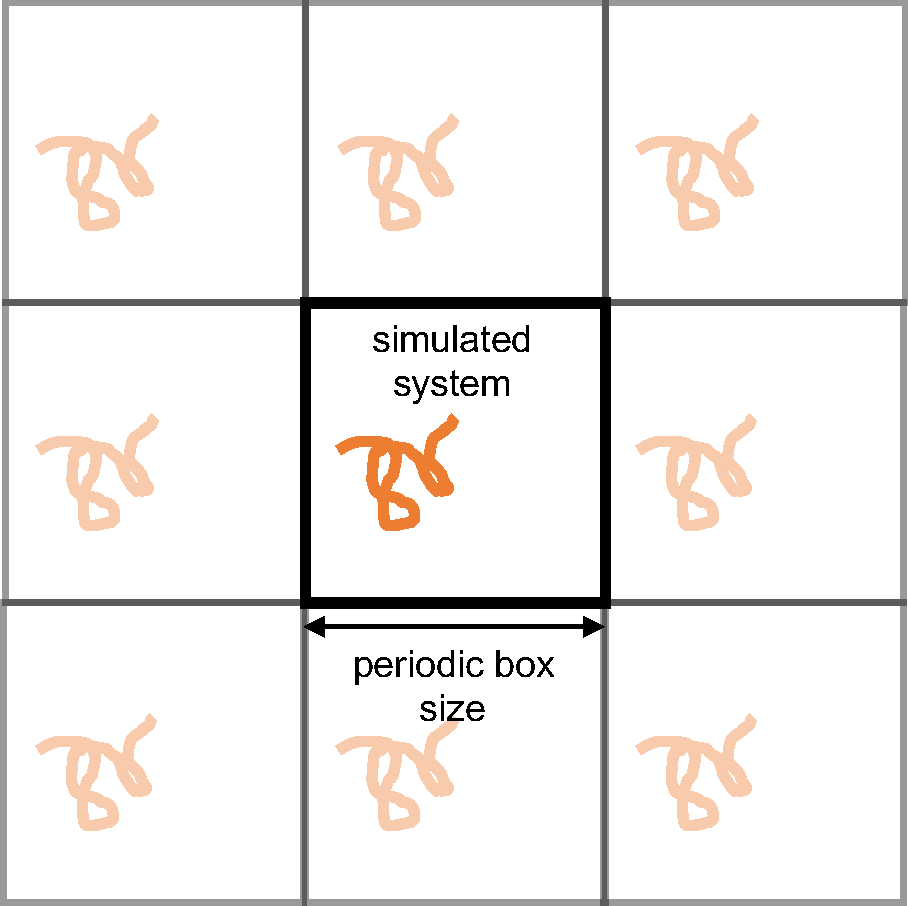
\includegraphics[width=\linewidth]{PBC_figure.pdf}
\caption{Periodic boundary conditions are shown for a simple 2D system. Note that the simulated system is a sub-ensemble within an infinitely sized system of identical, small ensembles.}
\label{pbcfig}
\end{figure}

Periodic boundary conditions allow more accurate estimation of bulk properties from simulations of finite, essentially nanoscale systems.
More precisely, simulations of comparatively small systems with periodic boundary conditions can be a good approximation to the behavior of a small subsystem in a larger bulk phase (or at least are a much better approximation than simply simulating a nanodroplet or a finite system surrounded by vacuum).
Periodic boundary conditions can alleviate many of the issues with finite size effects because each particle interacts with periodic images of particles in the same system.
Clearly, though, it is undesirable for a single particle to interact with the same particle multiple times.
To prevent this, a cut-off of many non-bonded interactions should be chosen that is less than half the length of the simulation box in any dimension.
(However, as noted in Section~\ref{sec:classical_electrostatics} these cut-offs are not normally applied to electrostatic interactions because truncating these interactions induces worse artifacts than does including interactions with multiple copies of the same particle. 
Instead, what are often termed ``cut-offs'' that are applied to electrostatics are instead a shift from short-range to long-range treatments.)
Such cut-offs impose a natural lower limit to the size of a periodic simulation box, as the box must be large enough to capture all of the most significant non-bonded interactions.
Further information on periodic boundary conditions and discussion of appropriate cut-offs may be found in \citet{LeachBook}, sections 6.5 and 6.7 and \citet{ShellNotes}, lecture on Simulations of bulk phases.
%DLM: I have permission to migrate Shell's notes to GitHub, specifically to https://github.com/kofkeLab/Mol-Sim-Intro, so I should go ahead and prioritizing these particular notes there and then cite here.

It is very important to note that periodic boundary conditions are simply an approximation to bulk behavior.
They DO NOT effectively simulate an infinitely sized simulation box, though they do reduce many otherwise egregious finite-size effects.
This is most easily seen by imagining the placement of a solute in a periodic simulation box.
The solute will be replicated in all of the surrounding periodic images.
The concentration of solute is thus exactly one per the volume of the box.
Although proper selection of non-bonded cutoffs will guarantee that these solutes do not directly interact, they may indirectly interact through their perturbation of nearby solvent.
If the solvent does not reach a bulk-like state between solutes, the simulation will still suffer from obvious finite-size effects.

Macroscopic, lab-scale systems, or bulk systems, typically consist of multiple moles of atoms/molecules and thus from a simulation perspective are effectively infinite systems.
We attempt to simulate these by simulating finite and fairly small systems, and, in a sense, the very idea that the simulation cell is not infinite, but simply periodic, immediately gives rise to finite-size effects.
Thus, our typical goal is not to remove these completely but to reduce these to levels that do not adversely impact the results of our simulations.
Finite-size effects are particularly apparent in the electrostatic components of simulations, as these forces are inherently longer ranged than dispersion forces, as discussed in Section~\ref{sec:classical_electrostatics}.
One should always check that unexpected long-range correlations (i.e. on the length-scale of the simulation box) do not exist in molecular structure, spatial position, or orientation.
It should also be recognized that periodic boundary conditions innately change the definition of the system and the properties calculated from it.
Many derivations, especially those involving transport properties, such as diffusivity \citep{Yeh2004}, assume infinite and not periodic boundary conditions. 
\todo[inline, color={green!20}]{JIM: Other examples to cite? I think there's some examples also involving calculations of entropy, but I'll have to check this}
The resulting differences in seemingly well-known expressions for computing properties of interest are often subtle, yet may have a large impact on results.
Such considerations should be kept in mind when comparing results between simulations and with experiment.

\subsection{Main steps of a molecular dynamics simulation}
\label{sec:main_steps}
While every system studied will present unique challenges and considerations,
the process of performing a molecular dynamics simulation generally follows
these steps:

\begin{enumerate}
\item System preparation
\item Minimization/Relaxation
\item Equilibration
\item Production
\end{enumerate}

Additional explanations of these steps along with procedural details specific to a given simulation package and application may be found in a variety of tutorials \citep{LemkulTutorials} \citep{AmberBeginner}.
It should be noted that these steps may be difficult to unambiguously differentiate and define in some cases.
Additionally, it is assumed that prior to performing any of these steps, an appropriate amount of deliberation has been devoted to clearly defining the system and determining the appropriate simulation techniques.

System preparation is the most variable of these steps, and often requires unique tools for every system of interest.
It is highly recommended that best practices documents specific to this issue and to the type of system of interest be consulted.
If such documents do not exist, it may be that a freely-available tool for constructing such a system does in fact exist.
Examples include tools for constructing specific crystal structures, proteins, and lipid membranes.
\todo[inline, color={green!20}]{JIM: Include some tools to cite here}
The goal of all of these tools, and system preparation in general, is to create a representation of the system of interest that can be interpreted by the desired simulation package.
It is further desirable that this representation not vary too far from the known, equilibrium structure of the system at the thermodynamic state point of interest.
For instance, highly energetically unfavorable configurations of the system, such as blatant atomic overlaps, should be avoided.
However, for a force field that reliably reproduces the energetics of a system, a starting configuration that is close to equilibrium is only a time-saving convenience in that it greatly reduces the equilibration time and overall simulation length by preventing trapping in metastable states.

The purpose of minimization, or relaxation, is to find a local energy minimum of the starting structure so that the molecular dynamics simulation does not immediately "blow up" (i.e. the forces on any one atom are not so large that the atoms move an unreasonable distance in a single time step).
This involves standard minimization algorithms such as steepest descent.
For a more involved discussion of minimization algorithms utilized in molecular simulation, see \citet{LeachBook}, sections 5.1-5.7.

At the end of energy minimization, it is important to achieve a system configuration with small enough forces that the desired time-step will well-approximate the dynamics (see \citet{LeachBook}, section 7.3.4).
Such a configuration is a suitable starting point for molecular dynamics techniques.
However, this only represents a static set of positions, while the propagation of dynamics also requires a set of starting velocities.
These may be assigned in a variety of ways, but are usually randomly assigned to atoms such that the correct Maxwell-Boltzmann distribution at the desired temperature is achieved.
Even though velocities are assigned according to the correct distribution, the selected thermostat will still usually need to add heat to or remove heat from the system as it approaches the correct partitioning of kinetic and potential energies.
For this reason, it is advised that a thermostatted simulation is performed prior to a desired production simulation, even if the production simulation will ultimately be done in the NVE ensemble.
Once the kinetic and potential energies fluctuate around constant values, the thermostat may be removed and a snapshot selected that is simultaneously as close to the average kinetic and potential energies as possible.
This snapshot, containing both positions and velocities may be used to then start an NVE simulation that will correspond to a temperature close to that which is desired.
This is necessary due to the fact that only the average temperature is obtained through coupling to a thermostat (see the below section on Thermostats), and the temperature fluctuates with the kinetic energy at each time step.
Similarly, equilibration in the NPT ensemble is necessary before production in the NVT if an average density consistent with a specific pressure is desired.
In this case, the system may be scaled to the desired average volume before the production simulation.
In the above example, the NPT simulation is said to have equilibrated to a specific volume when the dimensions of the simulation box fluctuate around constant values with minimal drift. 
This definition, though not perfectly rigorous, is usually suitable for assessing the equilibration of energies, temperature, pressure, and box dimensions during equilibration simulations.
The schematic below (\ref{eqworkflow}) demonstrates what is generally an appropriate equilibriation work-flow for common production ensembles.
Clearly, this schematic cannot cover every case of interest, but should provide some idea of the general approach.
For more information on equilibration procedures, see \citet{LeachBook}, section 7.4 and \citet{ShellNotes}, lectures on Molecular dynamics and Computing properties.
%DLM: Should we be saying something here about how long to equilibrate? My short version is "until the properties of the system stop changing on average", but there could be a whole set of properties one might want to look at. Clearly you should look at anything which is important to you, but also perhaps things which tend to be relatively slow, such as water, etc.
%JIM: I tried this out above.

\begin{figure}[h]
\centering
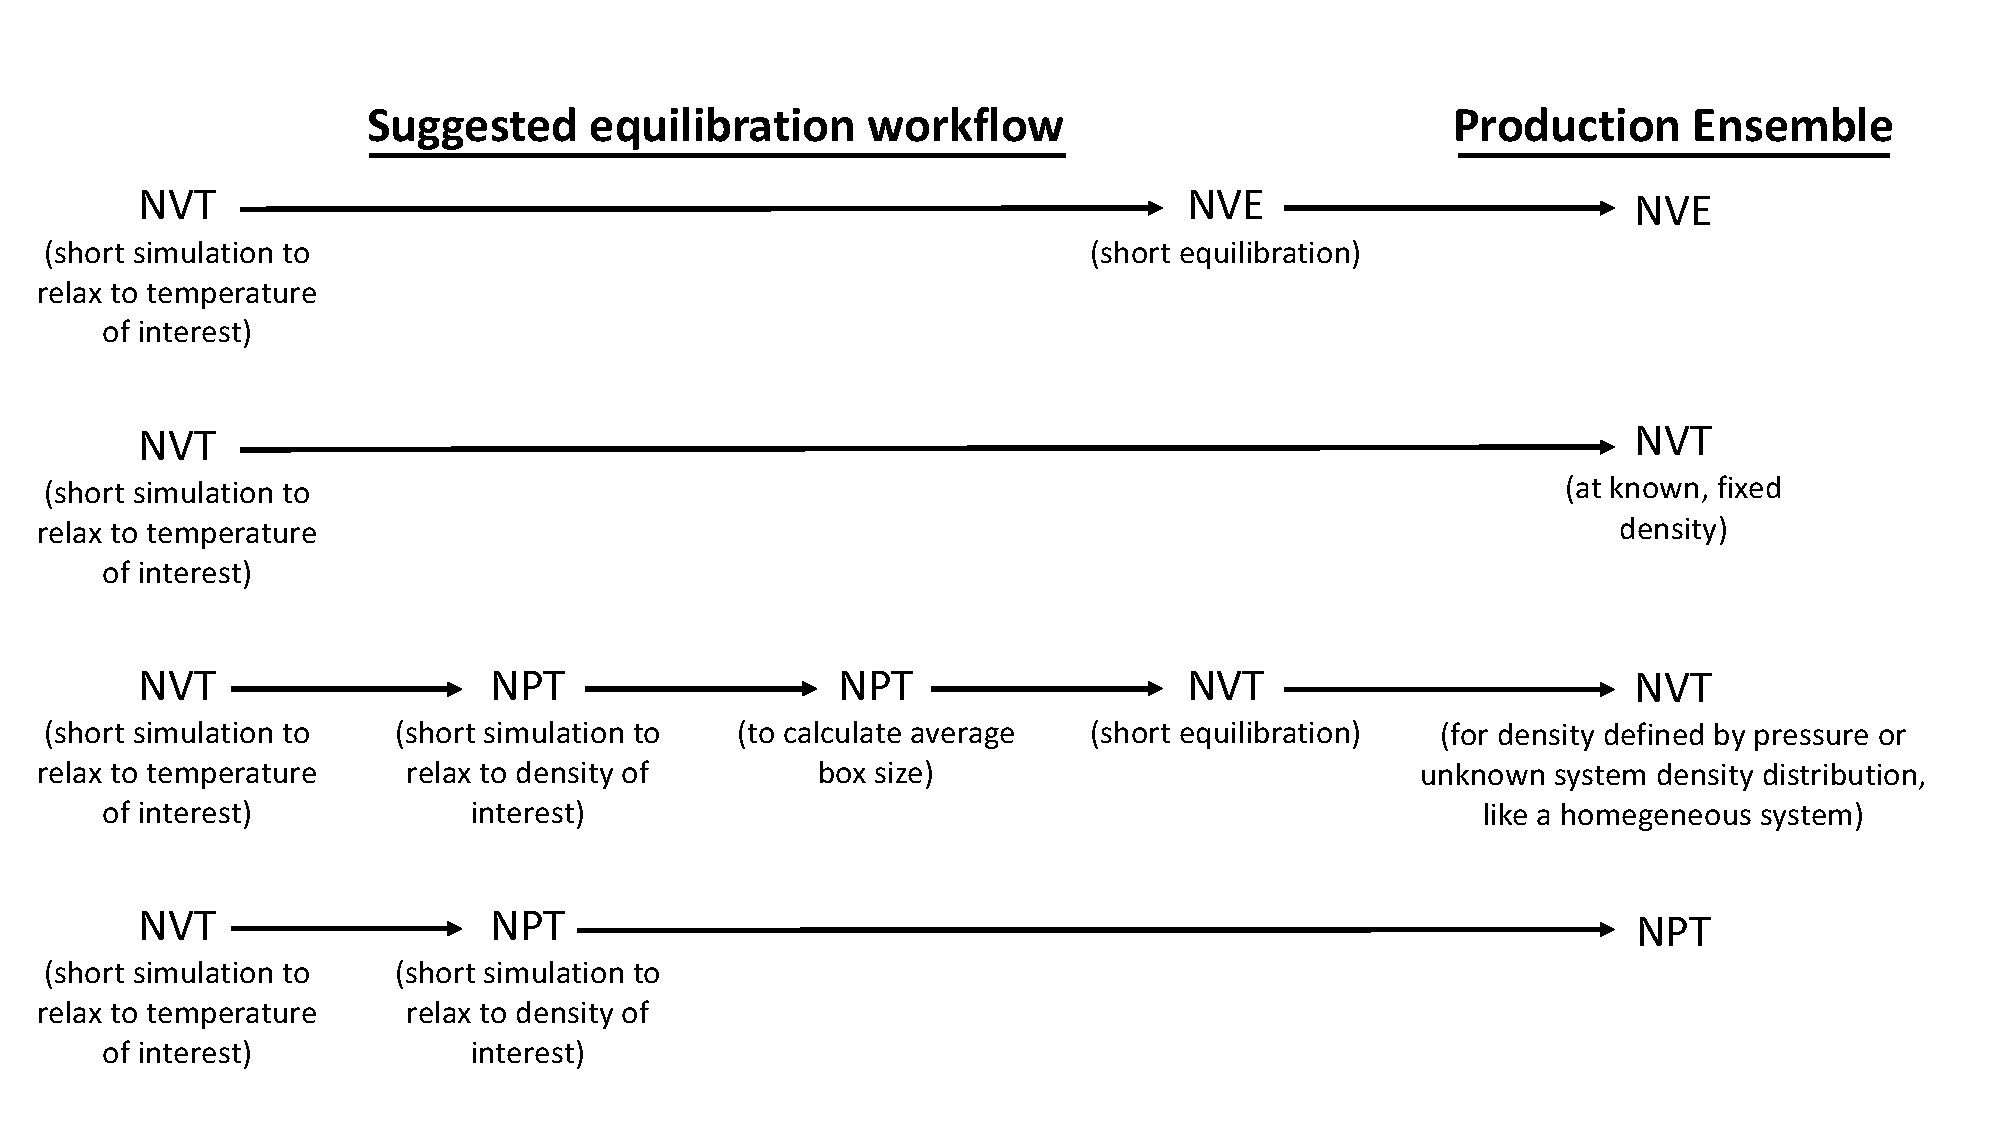
\includegraphics[width=\linewidth]{Equilibration_Workflow.pdf}
\caption{Common equilibration work-flows}
\label{eqworkflow}
\end{figure}

Once equilibration is complete, the production simulation may be performed.
The production simulation is that from which specific properties of the system of interest will be calculated.
As mentioned above, the equilibration procedure should be selected that is appropriate for the desired production ensemble.
It should be noted that ``equilibration'' within the production run may still be necessary before properties or metrics are computed from this simulation (see \citet{ShellNotes}, lecture on Computing properties).
%DLM: See comments above about migrating to GitHub/citing.
This falls under the category of correctly obtaining unbiased statistics and
convergence, which is covered in another best-practices document. %How to cite?
Do we even cite this?
%SHould cite; we can ask Zuckerman as I think he's in charge of that. Or Zuckerman and SHirts, as Shirts should have the overall list.
Otherwise, if a brief simulation in the same ensemble is not performed during the equilibration step immediately prior to production, any period of the production simulation should be ignored where drift is observed in the energies, temperatures, pressures, densities, or other defining state-variables of the ensemble.
This of course preceeds estimation of convergence in property calculation.
For more specific details on procedures and parameters used in production simulations, see the appropriate best practices document for the system of interest.

\subsection{Thermostats}
\label{sec:thermostats}
\begin{itemize}
\item Motivation
\item What is it?
\item Brief description of how it works
\item Popular thermostats
\end{itemize}

% Motivation for using thermostats
\subsubsection{Motivation}
As mentioned throughout the article above, molecular dynamics simulations are used to observe and glean properties of interest from some system of
study.
However, these properties traditionally are not measurable from the initial configuration of the system, nor is that usually physically meaningful.
This generally requires transitioning the system to some other state point to collect the proper data once the system has equilibrated.
In many cases, to emulate experiment, sampling from the canonical (constant-temperature) ensemble is desired\cite{thermostatAlgorithms2005}.
Generally, if the temperature of the system must be changed during the simulation, some thermostat algorithm will be employed. 
This section will review the background information about thermostats and how they work, some popular thermostats, and common issues to understand and avoid when using thermostats in MD simulations.

% relevant background information needed to understand thermostats
\subsubsection{Background and How They Work}
The difference between the types of temperatures that are measured in a simulation is important to know.
There is the target temperature, a temperature value that the system attempts to average about.
When specifying a temperature to thermostat to, this is the target temperature.
However, due to the fluctuations, it is not guaranteed that the temperature measured at singular point in time will be the target temperature.
Called the kinetic temperature, or instantaneous temperature, this value is derived from the equipartition theorem usually.
It should be noted that this value can be greater than, less than, or equal to the average kinetic energy.
The kinetic temperature should also be paid special attention to when describing the system.
The kinetic temperature does \textbf{not} state ``the temperature is at some value $T$'', it merely states: ``the energy of the system is similar to that
of a system at temperature $T$''.

Finally there are generally three types of thermostats: deterministic, stochastic, and extended system.
Deterministic thermostats are usually known to scale the momenta or forces on the particles in the system based on their fitness to the target temperature.
Stochastic thermostats behave similarly to the deterministic thermostats, however, there is a random force or momenta sampled out of a probability distribution that can scale or modify these properties of selected particles.
Extended system thermostats are similar to what their name suggests, the system has an added variable that has a degree of freedom.
This emulates an external heat bath that can interact with the particles in the system affecting their momenta in a predictable fashion.

\subsubsection{Popular Thermostats}
Within this section, various thermostats will be briefly explored, with a small description of their uses and possible issues that are associated with each.
This is by no means an exhaustive study of available thermostats, just some of the more popular and historic thermostats used in MD.

\subparagraph{Deterministic Thermostats}
\begin{enumerate}[listparindent=\parindent]
    \item \textbf{Velocity Rescaling}

        The velocity rescaling thermostat is one of the simplest thermostats to implement, however, this thermostat is also one of the most non-physical thermostats as well.

         This thermostat relies on rescaling the momenta of the particles every $N$ timesteps based on their ratio of the instantaneous temperature to the target temperature\cite{thermostatAlgorithms2005}. 
         This leads to multiple issues when trying to sample data using this thermostat.
         First, this method is not reversible, there lacks a way for the particles to have knowledge of their previous thermal history.
         This makes any dynamical value impossible to measure (diffusion for example). 
         There is also no distribution of momenta; this thermostat does not sample the canonical distribution and cannot be used for sampling at thermal equilibrium.

    \item \textbf{Hoover (Gaussian)}
        
        This thermostat is also an example of a velocity rescaling thermostat; however, the goal of the Gaussian thermostat is to ensure the change in
        temperature $\Delta T$ is always 0 ($\Delta T \equiv 0$).
        The reasoning for the naming of this thermostat is due to the method to solve for the smallest perturbative forces needed to keep the change in temperature equal to 0.
        Using the Gaussian principle of least constraint, forces are calculated to maintain a net 0 change in temperature, while minimally perturbing the system\cite{thermostatAlgorithms2005}.

        Important information to know about this thermostat is that it is reversible and canonical; however, there are no temperature
        fluctuations.
        This once again will lead to issues when trying to sample any properties from the canonical ensemble.
        Also, due to the nature of the thermostat preventing a change in temperature, whatever temperature
        the system is at when the thermostat is applied, it will stay there. 

    \item \textbf{Berendsen}

        The Berendsen thermostat is another type of velocity rescaling thermostat, but instead of the rescaling happening
        very abruptly each force adjustment time, we include a relaxation term to allow the system to more slowly approach the target
        temperature\cite{berendsen1984molecular}.
        With the introduction of a coupling parameter $\tau$, the strength of this parameter will determine
        how fast the system will approach the target temperature.
        However, it should be noted that while allowing for temperature fluctuations, the Berendsen thermostat is not canonical nor is it reversible.

\end{enumerate}

\subparagraph{Stochastic Thermostats}
\begin{enumerate}[listparindent=\parindent]
    \item \textbf{Andersen}

        The Andersen\cite{andersen1980molecular} thermostat is the first of two stochastic thermostats that will be explored.
        This thermostat has vestiges of the rescaling thermostats mentioned earlier, but with a randomization element also included.
        In this case, the Andersen thermostat attempts to model a system that is coupled to some random
        degree of freedom\cite{andersen1980molecular, thermostatAlgorithms2005}.
        In this case, this random element will be a new set of velocities that are chosen from a probability distribution and then if the reassignment probability passes, the velocities of the particle will be replaced.
        The number of particles affected, time between "collisions", and how often this is applied to the system are possible variations of this thermostat.
        Like the previous thermostats, this is not reversible, but the Andersen thermostat does reproduce the canonical ensemble.
    
    \item \textbf{Langevin}

        The Langevin\cite{schneider1978molecular} thermostat applies the idea of an implicit solvent as a way to randomly impart or remove some force acting on the particles. 
        With a general equation of the form $F = F_{interaction} + F_{friction} + F_{random}$, where $F_{interaction}$ is the standard interactions calculated during the course of the simulation, $F_{friction}$ is the damping parameter used to tune the  ``viscosity'' of the implicit bath, and $F_{random}$ is a random force perturbing the forces on the particles. 
        Careful consideration must be taken when choosing the friction damping parameter.


\end{enumerate}

\subparagraph{Extended System Thermostats}
\begin{enumerate}[listparindent=\parindent]

\item {\bf Nos\'{e}-Hoover}

   The Nos\'{e}-Hoover thermostat~\cite{thermostatAlgorithms2005} essentially abstracts away the thermal bath from the previous thermostats and condenses it into a singular additional degree of freedom.
    This bath with a ``mass'' that can be changed can interact with the particles in the system in a predictable and reproducible way while maintaining the
    canonical ensemble.
    This is one of the most widely implemented and used thermostats due to these attributes.
    However, it should be noted that with small enough systems, ergodicity can be an issue and the thermostat might not properly sample the canonical ensemble \cite{martyna1992nose,thermostatAlgorithms2005}. 
    This can become important even in systems with larger numbers of particles if a portion of the system does not interact strongly with the remainder of the system, such as in alchemical free energy calculations when a solute or ligand is non-interacting.
    
    
\item {\bf Nos\'{e}-Hoover Chain}

    Briefly mentioned above, there are certain conditions where the Nos\'{e}-Hoover thermostat might not be sufficient to properly sample the system, due to
   system size and ergodicity issues\cite{martyna1992nose, thermostatAlgorithms2005}. 
    However, Martyna et. al.  \cite{martyna1992nose} discovered that by coupling more heat baths to the system, the canonical ensemble can be rediscovered, at the minimal increase in computations required. In certain situations, it will be useful to chain additional heat baths to the system when under the Nos\'{e}-Hoover thermostat.

\end{enumerate}


\subsubsection{Summary}
To summarize, observe (\ref{tstat_summary}), as a general summary and guide for exploring the usage of various thermostats. Make sure to pay special attention to the reversibility when measuring time dependent properties, the ensemble sampled for all cases, and if a proper distribution of momenta and kinetic energy fluctuations are supported.
Do note that depending on the system of interest, it might not be necessary to worry about some of this information when initializing the system for a production run.
For example, if the thermal history of the system is not necessary during equilibration, a faster algorithm like Andersen or Berendsen could possibly be implemented, then switch to Nos\'{e}-Hoover when at the production run.
Knowing the system you are simulating and the benefits and weaknesses to each thermostat is crucial to successfully and efficiently collect meaningful, physical data.

\begin{figure}[h]
\centering
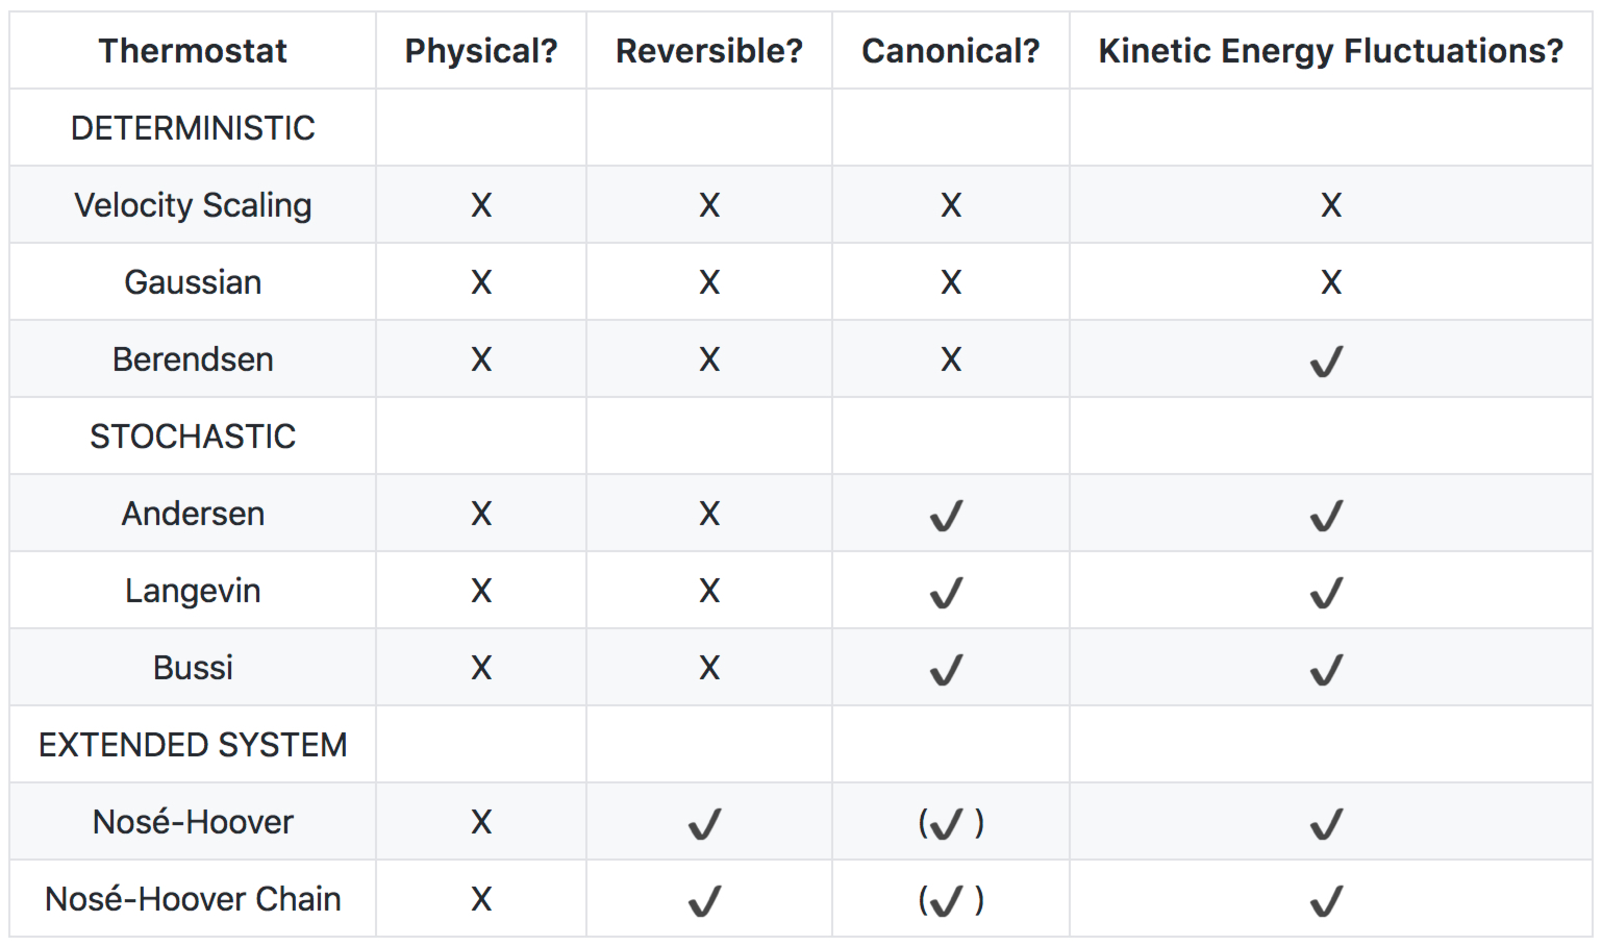
\includegraphics[width=\linewidth]{thermostat_summary.pdf}
    \caption{Basic summary of popular thermostats, where \ding{55} signifies
    that the thermostat does not fulfill that statement, \ding{51} does, and
    (\ding{51}) does under certain circumstances.}
\label{tstat_summary}
\end{figure}

\subsection{Barostats}
\label{sec:barostats}
\begin{itemize}
\item What is it?
\item Brief description of how it works
\item Popular barostats
\end{itemize}

\subsection{Integrators}
\label{sec:integrators}
\begin{itemize}
\item Numerical solution of dynamical equations of motions
\item Importance of energy conservation
\item Commonly used integrators
\item How to choose an appropriate timestep?
\end{itemize}

\subsection{Long range electrostatics}
\label{sec:lr_electrostatics}
\begin{itemize}
\item Cut-off is bad
\item Need for special treatment
\item Idea of an Ewald sum
\item PPPM
\item How to choose parameters
\end{itemize}

\begin{Checklists*}[p!]

\begin{checklist}{Take stock of your plans}

\begin{itemize}
\item \textbf{Count the cost: } Think about what you know about the timescales of what you want to observe and determine whether it is tractable to simulate this given the size of your system, your computational resources, and the expense of the simulation.
\item Pick the desired ensemble ($NVT$, $NPT$, $NVE$, $\mu VT$, $\mu PT$)
\item Determine reference states that you are trying to emulate/discover.
\item What temperature, pressure, etc. are you interested in?
\item What is already known in the literature and what data do you wish to compare to?
\end{itemize}
\end{checklist}

\begin{checklist}{Prepare to implement your plans and make critical decisions about system type}

\begin{itemize}
\item Choose a simulation package suitable for simulating that ensemble (see best practices document) % link
\item Determine whether you are simulating a bulk (typically periodic) or finite system and choose the appropriate cutoff types and periodicity (full periodicity for bulk systems, partial periodicity for interfaces, etc.) as discussed in [section] % reference section whatever
\end{itemize}
\end{checklist}

\begin{checklist}{Determine handling of cutoffs}
\begin{itemize}
\item As a general rule, electrostatics are long-range enough that either the cutoff needs to be larger than the system size (for finite systems) or
periodicity is needed 
\item Nonpolar interactions can often be safely treated with cutoffs of 1-1.5 nm as long as the system size is at least twice that, but long-range dispersion corrections may be needed
\end{itemize}
\end{checklist}

\begin{checklist}{Choose appropriate settings for the desired ensemble:}
\begin{itemize}
\item Pick a thermostat that gives the correct distribution of temperatures, not just the correct average temperature
\item Pick a barostat that gives the correct distribution of pressures
\item Consider the known shortcomings and limitations of certain integrators and thermostats/barostats and whether your choices will impact the properties you are calculating
\end{itemize}
\end{checklist}


\begin{checklist}{Choose an appropriate timestep for stability and avoiding energy drift}
\begin{itemize}
\item This depends on factors such as the use of constraints in the system (e.g. for all-atom systems constraining hydrogen bonds can allow the use of a slightly longer timestep; 2 fs is relatively typical)
\end{itemize}
\end{checklist}


\end{Checklists*}







\nocite{*}
\bibliography{basic_training}{}

\end{document}
